\documentclass[10pt]{article}
\usepackage[margin=1in]{geometry}
\usepackage{amsmath,amssymb}
\usepackage{booktabs}
\usepackage{graphicx}
\usepackage{xcolor}
\usepackage[numbers,sort&compress]{natbib}
\usepackage{caption}
\usepackage{float}
\usepackage{tikz}
\usetikzlibrary{arrows.meta,positioning,shapes.geometric}
\usepackage[colorlinks=true,linkcolor=blue!60!black,citecolor=blue!60!black,urlcolor=blue!60!black]{hyperref}
\graphicspath{{artifacts/figures/}}
\captionsetup{font=small,labelfont=bf}
\setlength{\parskip}{2pt}

\newcommand{\AF}{Anti-Filter Effect}
\newcommand{\CAA}{Counterfactual Abstain Attribution}
\newcommand{\SPC}{Signal Promotion Contract}
\newcommand{\id}[1]{\texttt{\small #1}}

\title{\textbf{When Abstention Destroys Alpha:\\ Counterfactual Abstain Attribution and Signal Promotion Contracts for Financial ML}}
\author{Zeb Freeman\\ \small Independent research; \texttt{trade\_bot} repository, ES futures and EUR/USD intraday systems}
\date{September 10, 2026}

\begin{document}
\maketitle

\begin{abstract}
Financial machine-learning pipelines commonly add an abstention layer (a confidence threshold, a regime veto, a reject option) on top of a classifier and promote the result when precision, F-scores, or average precision improve. We argue that this practice conflates two different objectives: a classifier estimates whether a trade will be labelled a success, while a trading system is paid for the net value of the trades it actually takes. We name the failure mode in which an abstention rule improves a predictive metric while lowering the declared economic utility of the strategy the \emph{\AF}, and we propose \emph{\CAA} (CAA) as the diagnostic: partition the baseline trades into accepted and rejected populations and measure the realized post-cost economics of both. Applied to 154 nested base-versus-abstain policy pairs and 139 trade-level re-screens saved in one research repository (three strategy families, ES futures and EUR/USD, 2012--2026), CAA finds that hard regime abstains raised event precision from 0.35 to 0.99 on the flagship EUR/USD model while removing 69\% of net profit, that the same abstains lowered net profit while raising precision in 45 of 49 walk-forward folds with rejected trades out-earning accepted trades per trade in aggregate, and that confidence-quantile filters on two ES branches removed 80--110\% of baseline profit. The effect is not universal: 43 of 96 walk-forward pairs are genuinely additive, and one branch is rescued by the same lever. Whether a quantile filter helps or hurts can depend on how its cutoff is computed, which is exactly the detail that differs between the research and live code paths. We formalize a \SPC\ that promotes a signal only after post-cost expectancy, additive value against the correct baseline, concentration safety, walk-forward robustness, replay parity of the exact deployable policy, and operational readiness are demonstrated.
\end{abstract}

\section{Introduction}

Supervised models in systematic trading are rarely deployed as bare predictors. A meta-labelling classifier scores each candidate setup, a threshold converts the score into a decision, and a rule stack may then veto the decision for reasons of regime, session, spacing, or confidence \citep{lopezdeprado2018,thumm2023}. Each of those layers is a form of selective prediction: the system trades on some candidates and abstains on the rest. Selective prediction has a mature theory in machine learning, from Chow's reject option \citep{chow1970} to selective classification with guaranteed risk \citep{elyaniv2010,geifman2017}, learning with rejection \citep{cortes2016}, and learning to defer \citep{madras2018,mozannar2020}. That theory measures success by the trade-off between \emph{coverage} (the fraction of inputs the model does not abstain on) and \emph{selective risk} (the error rate on covered inputs). Lower risk at lower coverage is, by construction, an improvement.

In a trading system that reading is wrong often enough to matter. The classifier's error rate is computed over labels; the strategy's performance is computed over money. A rejected candidate that would have been a labelled failure can still have been a profitable trade, and a correctly labelled success can lose money after costs. When the two orderings diverge, abstention can raise every classifier metric while lowering the strategy's net profit, and a promotion process that watches classifier metrics will promote the wrong policy. We call this the \emph{\AF}.

This paper does three things. First, it defines the \AF\ relative to an explicitly declared economic utility, and shows that its presence is decided by one quantity that is almost never reported: the realized post-cost value of the trades the filter rejected. Second, it introduces \CAA\ (CAA), a small, auditable procedure for computing that quantity from artifacts a research pipeline already produces, and applies it to the saved experiments of one research repository. Third, it proposes a \SPC: a compact set of conditions under which a candidate model or filter may become a promoted trading signal, unifying gates the repository already had with the two conditions it lacked.

The empirical material is deliberately narrow and fully traceable. Every number in Sections~\ref{sec:setting} and~\ref{sec:results} is recomputed from a saved artifact by the scripts shipped with the paper, and every source file is listed with its SHA-256 digest. Where a claim rests on a journal note rather than a regenerated number, the text says so. We report negative and mixed results alongside the headline ones because the concept is only useful if it is not universal.

\section{Background and Motivation}

\subsection{Selective prediction in financial ML}

Let a candidate trade be described by features $x$ and a binary success label $y$ produced by a labelling rule (for example, a triple-barrier or fixed-horizon markout). A meta-labelling classifier estimates $p(x)\approx P(y=1\mid x)$. A decision policy $\pi$ maps $p(x)$ and context to \{trade, abstain\}. Following the selective-classification literature we write coverage as the fraction of eligible candidates on which the policy trades. Conventional practice evaluates $\pi$ with precision (the share of taken trades whose label is 1), recall, $F_\beta$, average precision (AP), ROC-AUC, or calibration, and treats a policy that raises precision at acceptable coverage as better. In the repository studied here the threshold search literally optimizes a score of $0.60\cdot F_{0.5}+0.40\cdot(\text{normalized post-cost expectancy})$, and the hard-abstain rules are applied downstream of it without any fitted objective (evidence map E24).

\subsection{Why classifier improvement can differ from economic improvement}

Let $v_i$ denote the realized net value of trade $i$ after spread, slippage, and commission. The trading system's objective is a functional of the multiset $\{v_i\}$ of taken trades: total net PnL, expectancy (mean $v_i$), a risk-adjusted ratio, or a drawdown-constrained return. The classifier's objective is a functional of $\{(p_i,y_i)\}$. These agree only if $v_i$ is a fixed function of $y_i$, which fails for at least four reasons present in our data:
\begin{enumerate}\setlength{\itemsep}{0pt}
\item \textbf{Payoff asymmetry and magnitude.} With a 2:1 target-to-stop geometry a 45\% hit rate is profitable and precision-destructive; with fixed-horizon markouts a labelled failure can close at a small profit and a labelled success at a small loss after costs. Trade magnitudes vary by an order of magnitude within one tape.
\item \textbf{Rare large winners.} On thin event sets one trade can be most of the profit. In the ICT short-continuation branch below, one trade with model probability $0.555$ against a $0.55$ threshold is 78\% of baseline net PnL; any confidence filter removes it.
\item \textbf{Weak or mis-ordered scores.} Several branches have ROC-AUC of $0.52$--$0.60$ and AP lift over the base rate below $0.07$ (E23). Their probabilities cluster within a few hundredths of the threshold, so ``more confident'' is barely distinguishable from noise, and realized expectancy is non-monotone in the score (Figure~\ref{fig:quintiles}).
\item \textbf{Regime and cost structure.} Hard abstains keyed to volatility state or session remove trades whose value is determined by the same state; nothing guarantees that the removed state was the unprofitable one.
\end{enumerate}
None of this is an argument against abstention. It is an argument that abstention is a decision policy whose economic effect must be measured, not inferred from a classifier metric.

\section{The Anti-Filter Effect}

\subsection{Definition}

Let $B$ be the set of trades produced by a baseline policy on an evaluation window, and let an abstention rule partition it into accepted trades $A$ and rejected trades $R$, with $B=A\cup R$, $A\cap R=\varnothing$. Coverage is $c=|A|/|B|$. For any trade set $S$ write $V(S)=\sum_{i\in S}v_i$ for net PnL, $e(S)=V(S)/|S|$ for expectancy, and $\pi(S)$ for a predictive quality measure (label precision, event precision, AP). Let $U(\cdot)$ be an \emph{economic utility declared before the experiment}; in this paper $U\in\{V,\,e,\,\text{monthly Sharpe subject to a drawdown limit}\}$ and the choice is always stated.

\begin{quote}
\textbf{Definition 1 (\AF).} An abstention rule exhibits the \AF\ with respect to $(\pi,U)$ if $\pi(A)>\pi(B)$ and $U(A)<U(B)$.
\end{quote}

Because $V(B)=V(A)+V(R)$ and $e(B)=c\,e(A)+(1-c)\,e(R)$, the two most common utilities reduce to statements about the rejected population:
\begin{equation}
U=V:\quad U(A)<U(B)\iff V(R)>0, \qquad\qquad U=e:\quad U(A)<U(B)\iff e(R)>e(A).
\label{eq:identity}
\end{equation}
In words: a filter destroys total profit exactly when the trades it rejected were net profitable, and it lowers expectancy exactly when the rejected trades were better per trade than the ones it kept. A filter can therefore raise expectancy and lower total profit at the same time (rejected trades profitable but below the accepted average); whether that is acceptable depends on capacity and risk constraints, which is why $U$ must be declared rather than assumed. The strict form of the effect, and the one we count in the censuses below, uses $U=V$; we report the expectancy form and saved risk-adjusted metrics alongside it.

\subsection{Counterfactual Abstain Attribution}

\CAA\ is the measurement that makes Definition~1 decidable. Given the baseline trade tape (one row per eligible trade with its realized net value, label, score, timestamp, and context) and the abstention rule, CAA reports for each of $B$, $A$, and $R$: count, coverage, gross and net PnL, expectancy, label precision, win rate, maximum drawdown, a monthly Sharpe proxy, and concentration (largest-winner, top-5, and top-10\% shares of net PnL); the deltas $U(A)-U(B)$; breakdowns of $A$ and $R$ by side, session, volatility regime, calendar year, fold, confidence band, label, and outcome; and the top contributors in each population. Two checks are part of the procedure rather than optional extras:

\begin{itemize}\setlength{\itemsep}{0pt}
\item \textbf{Nesting.} If the filtered policy can also \emph{add} trades (a cooldown that frees a slot, a regime threshold that lowers the bar elsewhere), then $A\not\subseteq B$ and the ``rejected'' economics are not a clean difference. CAA matches trades on an exact key, here \texttt{(entry\_datetime, source\_row\_idx)}, and reports the added set separately.
\item \textbf{Cutoff-rule sensitivity.} A data-dependent cutoff (``abstain below the 40th percentile of candidate probabilities'') is not a decision rule until the window over which the percentile is computed is fixed. CAA re-evaluates the same nominal rule under every window the pipeline could plausibly use at decision time.
\end{itemize}

The counterfactual assumption is the one already embedded in the research backtest: the rejected trade would have been filled at the modelled price and cost and its outcome is the labelled or marked-out outcome. No new simulation is required, because the outcome of every candidate was computed when the label was made. The assumption is weakest for trades whose presence changes others (concurrency, cooldown), which is what the nesting check is for.

\begin{figure}[t]
\centering
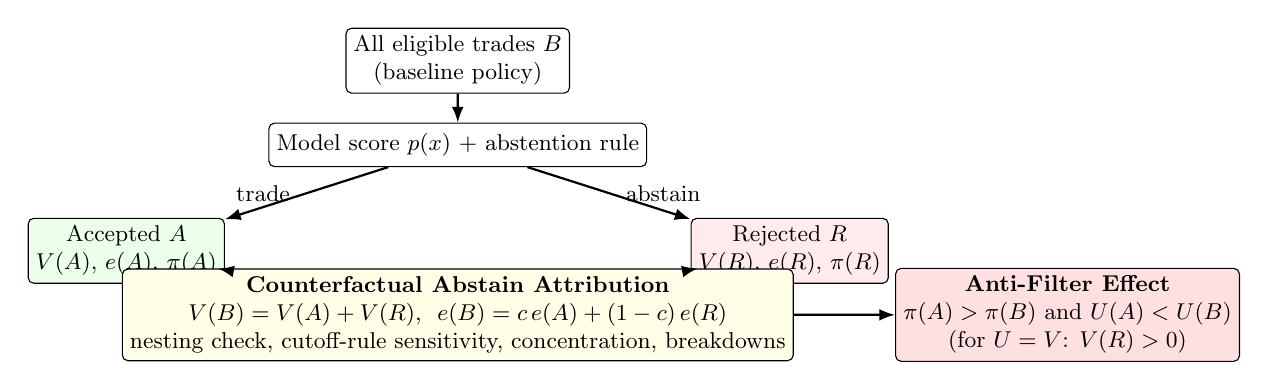
\begin{tikzpicture}[scale=0.92, transform shape, node distance=4mm and 8mm, every node/.style={font=\small}, box/.style={draw, rounded corners=2pt, minimum height=6mm, inner sep=3pt, align=center}, arr/.style={-{Latex[length=2mm]}, thick}]
\node[box] (b) {All eligible trades $B$\\ (baseline policy)};
\node[box, below=of b] (m) {Model score $p(x)$ + abstention rule};
\node[box, below left=7mm and 6mm of m, fill=green!8] (a) {Accepted $A$\\ $V(A),\,e(A),\,\pi(A)$};
\node[box, below right=7mm and 6mm of m, fill=red!8] (r) {Rejected $R$\\ $V(R),\,e(R),\,\pi(R)$};
\node[box, below=14mm of m, fill=yellow!10] (caa) {\textbf{Counterfactual Abstain Attribution}\\ $V(B)=V(A)+V(R)$,\ \ $e(B)=c\,e(A)+(1-c)\,e(R)$\\ nesting check, cutoff-rule sensitivity, concentration, breakdowns};
\node[box, right=14mm of caa, fill=red!12] (af) {\textbf{\AF}\\ $\pi(A)>\pi(B)$ and $U(A)<U(B)$\\ (for $U=V$: $V(R)>0$)};
\draw[arr] (b) -- (m);
\draw[arr] (m) -- node[left, xshift=-1mm]{trade} (a);
\draw[arr] (m) -- node[right, xshift=1mm]{abstain} (r);
\draw[arr] (a) -- (caa);
\draw[arr] (r) -- (caa);
\draw[arr] (caa) -- (af);
\end{tikzpicture}
\caption{The \AF\ and its diagnostic. Conventional evaluation looks only at the accepted population $A$. CAA measures the rejected population $R$ with the same economics and asks what the filter removed.}
\label{fig:schematic}
\end{figure}

\subsection{Economic failure modes}

Equation~\eqref{eq:identity} makes the possible failure modes concrete. (i) \emph{Alpha removal}: $V(R)>0$, the filter threw away profit. (ii) \emph{Quality inversion}: $e(R)>e(A)$, the filter kept the worse trades on average. (iii) \emph{Concentration transfer}: $A$ is smaller and one or a few trades now dominate $V(A)$, so the surviving strategy is more fragile even if $V(A)$ is higher. (iv) \emph{Structural shift}: $A$ and $R$ differ systematically by side, session, or regime, so the filter has changed the strategy's exposure rather than its quality. (v) \emph{Definition dependence}: the sign of $U(A)-U(B)$ changes with the cutoff window, so the research result is not a property of the deployable rule. (vi) \emph{Path divergence}: the research policy and the deployable policy are different objects and produce different $A$. All six occur in the evidence below; we say which.

\section{Experimental Setting}
\label{sec:setting}

\subsection{Strategies, instruments, and models}

The repository contains three event-driven intraday strategy families, each with a rule-based setup detector that emits candidate events and a meta-labelling classifier that scores them.

\begin{itemize}\setlength{\itemsep}{0pt}
\item \textbf{OTE} (Optimal Trade Entry): EUR/USD 5-minute bars, pullback-entry events, 120-bar label horizon, temporal convolutional networks (TCN) and XGBoost. The flagship is a long TCN (\id{long\_ote\_tcn\_v2}); test ROC-AUC 0.973, Brier 0.0066.
\item \textbf{FRVP} (fixed-range volume profile): ES futures 5-minute bars, six numbered setups pooled into continuation, reversal, and ``meta'' (all-setup) direction families, XGBoost and TCN. We also use one setup-specific lane (Setup 2 long continuation).
\item \textbf{ICT} (smart-money-concept setups: liquidity sweeps, fair value gaps, order blocks): ES futures 5-minute bars, continuation, reversal, and meta families, XGBoost trained with sequential bootstrap and event-window embargo.
\end{itemize}
The four branches on which the 2026-08-30 quantile study was run are the weak-discrimination branches identified by the repository's live signal audit (E23): FRVP short meta (test AP lift over base rate 0.014, ROC-AUC 0.525), FRVP long meta (0.067, 0.597), ICT long continuation (0.009, 0.534), ICT short continuation (0.059, 0.553).

\subsection{Labels, evaluation, and sample sizes}

All economics are computed on walk-forward test windows: three-month test folds stepped quarterly, a two-year minimum training span, a 40-bar purge gap between the training end and the test start, and, for ICT, a per-target embargo of 36--49 bars derived from realized event windows and verified with zero boundary failures (E27). Within each fold the global threshold, the per-regime threshold table, and the choice among four policy variants (\emph{global threshold}, \emph{regime threshold}, and each with the hard-abstain stack) are selected on the fold's training split and applied unchanged to the test window. Walk-forward efficiency (WFE) is test annualized PnL divided by train annualized PnL. The deflated Sharpe ratio (DSR) follows \citet{bailey2014dsr} with the recorded number of trials. A label-shuffle placebo for the FRVP continuation model gives out-of-fold AP 0.737 against $0.500\pm0.006$ over ten shuffles (E27).

Table~\ref{tab:samples} makes the distinction between bars and independent trading observations explicit. The largest tape has 6,514 trades; the ICT continuation tapes have 165 and 247. We make no significance claims for single-branch differences.

\begin{table}[t]
\centering\small
\caption{Sample-size ladder for the tapes analysed. Bars are 5-minute; ``usable events'' are labelled setup events after warm-up and ambiguity exclusion; trades are walk-forward test-window trades under the selected policy. Sources: training summaries, journal E13, saved backtest summaries (E32).}
\label{tab:samples}
\resizebox{\textwidth}{!}{%
\begin{tabular}{@{}lrrrrr@{}}
\toprule
Tape & bars / label rows & setup events & usable events (positives) & test trades & folds \\
\midrule
OTE long TCN v2 (EUR/USD) & 1,346,067 usable rows & -- & 21,954 positive rows & 6,514 & 49 \\
FRVP short meta (ES) & 666,769 & 28,667 (all setups) & 9,851 (4,733) & 1,523 & 25 \\
FRVP long meta (ES) & 666,769 & 28,667 & 9,349 (4,481) & 3,621 & 25 \\
FRVP long continuation (ES) & 666,769 & 28,667 & 6,608 (3,203) & 1,609 & 24 \\
FRVP Setup-2 long continuation (ES) & 666,769 & 28,667 & 999 (510) & 201 & 9 \\
ICT long continuation (ES) & -- & -- & 1,592 (813) & 247 & 18 \\
ICT short continuation (ES) & -- & -- & 1,277 (576) & 165 & 16 \\
\bottomrule
\end{tabular}}
\end{table}

\subsection{Transaction-cost assumptions}

ES: session-scheduled spread of 1.0 tick (overlap, London, New York), 1.5 (Asia), 2.0 (off-hours), plus 0.25 ticks slippage and 0.40 ticks commission per trade; one tick is 0.25 index points (\$12.50). EUR/USD: session spread 1.0/1.5/1.5/2.5/3.0 pips plus 0.3 pips slippage and 0.35 pips commission. Entry is the signal-bar close; exit is the label-horizon close (120 bars) or barrier. All PnL figures below are post-cost.

\subsection{Abstention policies studied}

Two families of abstention appear in the saved artifacts. The \emph{hard-abstain stack} vetoes candidates in high-stress volatility regimes, in the off-hours session, inside a four-bar cooldown after an accepted signal, and (when configured) in explicitly blocked regime/session pockets; it is evaluated in every backtest as the ``+abstain'' variant of each base policy, so the accepted set is nested in the base set and CAA is exact at the aggregate level. The \emph{probability-quantile filter} abstains on candidates whose calibrated probability is at or below the $q$-th quantile of candidate probabilities; it was evaluated on 2026-08-30 as a retrospective trade-level screen and, for a subset, as full candidate-level walk-forward reruns. In the research code the quantile is computed over the whole frame being evaluated (for a test decision, the entire three-month fold); in the live runtime it is computed over a rolling window of the last 512 candidate probabilities (E19). We evaluate three cutoff rules for the same nominal $q$: \emph{retrospective} (within the test fold, reproducing the 2026-08-30 screen), \emph{causal} (from the fold's saved training-window trades, knowable at fold start), and \emph{rolling} (from the previous 100 emitted trades, mimicking the live semantics).

\section{Results}
\label{sec:results}

\subsection{Baseline versus filtered performance}

Table~\ref{tab:headline} collects the headline comparisons. Columns give baseline, accepted, and rejected counts and economics; $\pi$ is event precision for the static OTE rows and label precision for tape-level rows; the class column applies Definition~1 with $U=V$ (AF: precision up and net down; PF: net up; ND: net down without a precision gain; suffix S: saved monthly Sharpe rose).

\begin{table}[t]
\centering
\caption{Headline \CAA. $N$ counts trades, $\pi$ precision, $e$ expectancy (per trade), $V$ net PnL; subscripts $B$ (baseline), $A$ (accepted), $R$ (rejected). Units are pips for OTE rows and ES ticks otherwise. Static rows are the 2026-04-03 and 2026-05-28 held-out test splits; all other rows are walk-forward runs matched on the exact trade key. Class: AF = \AF\ ($\pi\uparrow$, $V\downarrow$), PF = pro-filter ($V\uparrow$), ND = net down without precision gain, +S = saved Sharpe rose.}
\label{tab:headline}
\resizebox{\textwidth}{!}{\input{artifacts/tables/headline_attribution.tex}}
\end{table}

\paragraph{Hard abstains on the flagship EUR/USD model.} On the static held-out test the long TCN v2 emits 1,801 candidate trades under its searched global threshold and 630 once the hard-abstain stack is applied; event precision rises from 0.354 to 0.987 and event $F_{0.5}$ from 0.382 to 0.846, but net PnL falls from 14,573 to 4,469 pips. The 1,171 rejected trades carried 10,104 pips at 8.6 pips per trade, against 7.1 for the accepted trades. The same pattern holds for all eight static pairs on the four TCN-focus models and, in the walk-forward, fold by fold: over 49 quarterly folds the abstain variant is an anti-filter in 45 (long v2, global base) and 47 (regime base); the rejected population is 4,096 trades and 39,004 of 53,644 pips, with rejected expectancy 9.5 versus accepted 5.9 pips (E01--E03). The repository's framework paper recorded the aggregate as ``a blunt trade suppressor'' and an internal diagnostic note had already called the layer an anti-filter; CAA turns that reading into a per-fold, per-population measurement.

\paragraph{Confidence-quantile filters on weak ES branches.} For FRVP short meta, the candidate-level walk-forward rerun with $q=0.10$ and $0.20$ raised label precision from 0.534 to 0.537 and 0.546 and cut net PnL from $+1{,}995$ to $+20$ and $-215$ ticks; the rejected trades carried $+1{,}974$ and $+2{,}210$ ticks at 4.0 and 3.3 ticks each (E06). For ICT short continuation, $q=0.50$ and $0.60$ raised precision from 0.521 to 0.566 and 0.574 and cut net PnL from $+501$ to $+49$ and $+102$ ticks; the rejected trades carried $+452$ and $+398$ ticks (E08). In both cases the accepted population is ``more selective and more accurate'' in exactly the sense the selective-classification literature would reward, and the strategy is economically worse.

\paragraph{When the filter is additive.} The same lever rescues ICT long continuation: $q=0.40$ turns a flat branch (247 trades, $+7$ ticks) into 107 trades and $+499$ ticks with Sharpe 0.93 and WFE 0.98; the rejected trades lost 492 ticks, and the sign is stable across all 18 trade-level cutoff variants (E11). Regime/session pocket prunes on frozen FRVP models are additive in two of three cases and, in the long-meta case, spectacularly so: 3,062 rejected trades lost 13,651 ticks while label precision \emph{fell} from 0.505 to 0.491 (E12). Precision and economics decouple in both directions.

\subsection{Counterfactual economics of abstained trades}

Figure~\ref{fig:pairs} plots every nested pair in the two censuses. Of 96 walk-forward pairs, 83 raise precision; 40 are anti-filters and 43 are pro-filters under $U=V$. Of 58 static pairs, 29 are anti-filters and 21 pro-filters. In the walk-forward OTE pairs the rejected trades out-earn the accepted trades per trade in 19 of 36 comparisons (Table~\ref{tab:census}). The pattern is sign-conditional on the baseline: hard abstains remove profit on the profitable branches (short reversal XGB v2 in eight of eight folds, long reversal TCN in seven of eight, long meta and long union in a majority of folds) and reduce losses on the unprofitable ones (the breakout models, the static short meta and union branches), which is what a throughput suppressor uncorrelated with trade value would do (E29; the per-rule attribution that would confirm the mechanism was never run, E30).

\begin{table}[t]
\centering\small
\caption{Census of nested base-versus-abstain comparisons and trade-level quantile re-screens. ``$e_R>e_A$'': rejected expectancy exceeds accepted expectancy. Comparisons share trades and folds and are not independent trials.}
\label{tab:census}
\resizebox{\textwidth}{!}{\input{artifacts/tables/census.tex}}
\end{table}

\begin{figure}[t]
\centering
\includegraphics[width=0.62\textwidth]{policy_pair_scatter.pdf}
\caption{Change in event precision versus change in net PnL (relative to the baseline's absolute net PnL) for 154 nested policy pairs. The shaded quadrant is the \AF. OTE hard abstains cluster at large precision gains; FRVP and ICT pairs cluster near zero precision change with economic effects of either sign.}
\label{fig:pairs}
\end{figure}

\paragraph{Structure of the rejected population.} The breakdowns show what the filters removed. For ICT short continuation at $q=0.60$ the rejected set holds the branch's largest winner ($+391$ ticks on 2025-01-31, probability 0.555 against a 0.55 threshold), a positive New York pocket ($+443$ ticks over 27 trades), and 2022's profit ($+238$ over 12 trades at 75\% label precision), while the accepted set keeps a losing Asia pocket. For FRVP short meta at $q=0.20$ the rejected set is concentrated in the London/New York overlap session ($+2{,}266$ ticks over 62 trades, 36.5 per trade, versus 12.4 for the accepted overlap trades) and in 2021--2022. These are structural shifts, not uniform thinning, and neither would have been visible from the accepted population alone.

\subsection{Cutoff definition, concentration, and regime effects}

Table~\ref{tab:cutoff} and Figure~\ref{fig:coverage} show the trade-level re-screens under the three cutoff rules. For ICT short continuation the accepted population is net negative or within a few ticks of zero at \emph{every} quantile when the cutoff comes from the fold's training window ($-196$, $-85$, $-26$, $-80$, $-235$, $-3$ ticks for $q=0.1$ to $0.6$); the $+530$ result at $q=0.60$ that motivated the walk-forward rerun exists only under the retrospective and rolling cutoffs. For FRVP short meta the same nominal $q=0.10$ yields $+1{,}592$, $+1{,}611$, and $+5{,}096$ ticks under the three rules against an $1{,}829$ baseline, and $q=0.20$ yields $+1{,}076$, $+3$, and $+4{,}473$. The sign of the filter's effect is a property of the cutoff window, not of the model, and the window used in the saved research runs (within the test fold) is not the one the live code implements (E09, E10, E19).

\begin{table}[t]
\centering\small
\caption{Accepted-population net PnL for the same nominal quantile under three cutoff rules (ES ticks). Retrospective: quantile of the test fold's own emitted probabilities (the 2026-08-30 screen). Causal: quantile of the fold's saved training-window trades. Rolling: quantile of the previous 100 emitted test trades.}
\label{tab:cutoff}
\resizebox{\textwidth}{!}{\input{artifacts/tables/cutoff_sensitivity.tex}}
\end{table}

\begin{figure}[t]
\centering
\includegraphics[width=\textwidth]{coverage_profit_curves.pdf}
\caption{Coverage--profit curves: accepted net PnL relative to the baseline's absolute net PnL, as coverage is reduced by each cutoff rule. The horizontal line is the baseline. A pro-filter sits above the line; an anti-filter below it. Note the ICT long-continuation baseline is only 7 ticks, so its ratio scale is large. Absolute-probability thresholds collapse to a handful of trades on the ES branches because their probabilities cluster within 0.05 of the threshold.}
\label{fig:coverage}
\end{figure}

Concentration cuts both ways. The ICT short-continuation baseline is itself fragile (largest-trade share 0.78), and the filters that lower its profit do so mainly by removing that trade; neither the baseline nor any quantile variant passes the 10\% largest-trade gate. The additive ICT long-continuation $q=0.40$ result carries a largest-trade share of 0.249 and top-five share of 66\%; five pocket-control variants stacked on it reach at best 0.136 (E11). On the FRVP recent-regime reversal lane the accepted sparse-pocket prune rejected 11 trades carrying $+517$ ticks (net $-12\%$, Sharpe 1.43 $\to$ 1.48) and was adopted because the largest-trade share fell from 0.128 to 0.0999, just under the limit; under the fixed live contract the share was 0.1287 again (E14, E17).

Figure~\ref{fig:quintiles} shows why a threshold on the score is a sound control for some branches and not others. Expectancy rises monotonically with confidence quintile for the OTE long TCN (3.6 to 11.9 pips) and roughly so for the ICT reversal branches; for FRVP long continuation the top quintile earns 4.1 ticks against 12.0 in the bottom quintile, for FRVP long meta the top quintile is the worst, and for ICT short continuation the bottom quintile is the best. Where the score does not order value, confidence abstention cannot be expected to select it.

\begin{figure}[t]
\centering
\includegraphics[width=0.92\textwidth]{confidence_quintiles.pdf}
\caption{Post-cost expectancy by within-tape confidence quintile on walk-forward test trades. Left column: score orders value. Right two columns: it does not. Quintiles are pooled across folds, so the probability scale may drift within a quintile.}
\label{fig:quintiles}
\end{figure}

\subsection{Replay and robustness findings}

Table~\ref{tab:parity} compares the research-time adaptive walk-forward (a mixture of per-fold policies) with the exact fixed policy that would be deployed, on the same frozen predictions. For FRVP long continuation the adaptive result passes all eight gates (512 trades, $+7{,}001$ ticks, Sharpe 1.19); the fixed global-0.70 contract yields 180 trades, $+2{,}473$ ticks, Sharpe 0.74, and fails three gates. For the recent-regime reversal contract the fixed policy retains most of the economics but loses the concentration pass. Feature replay matched 96 of 96 cells and persisted prediction and decision replay matched exactly for the FRVP bundle; for the ICT bundle prediction replay matched 150 rows per model with zero mismatches and feature replay matched 405 of 414 cells, the 9 mismatches being raw coordinate features that shift the shadow reversal model's probability by 0.004--0.005 and block its promotion (E17, E18). Live confirmation windows for both bundles are authorized but had not started at the time of writing because the collector heartbeat was stale (E31).

\begin{table}[t]
\centering\small
\caption{Policy parity on frozen FRVP predictions (ES ticks). The adaptive walk-forward selects a policy variant per fold on the training split; the fixed live contract applies the packaged static policy to every fold. Source: paper-signal bundle run summary, 2026-08-16.}
\label{tab:parity}
\resizebox{\textwidth}{!}{\input{artifacts/tables/parity.tex}}
\end{table}

Two further robustness observations. First, a classifier can be excellent and worthless: the breakout-sustained pilot has cross-validated AP 0.982, test AP 0.996, and ROC-AUC 0.9999, and loses 2,646 pips over 789 walk-forward trades (E20). Second, the same registry entry evaluated seven weeks apart produced 1,523 and 1,713 baseline trades ($+1{,}829$ and $+1{,}995$ ticks) for FRVP short meta; the cause is not recorded (E28). Both are reasons to make replay parity and artifact pinning explicit promotion conditions rather than good habits.

\section{Signal Promotion Contract}

The repository already had an eight-gate acceptance contract (post-cost profitability, monthly Sharpe $\ge 0.80$, WFE $>0.50$, DSR $\ge 0.30$, profitable-quarter share $\ge 0.60$, positive-composite-expectancy share $\ge 0.60$, largest-single-trade share $<0.10$, account drawdown $<12\%$ advisory), a promotion-quality mode (3 trades per week, minimum fold counts, no auto-relaxed folds), a label-shuffle placebo, roll audits, and feature/prediction/decision replay audits with SHA-256-pinned bundles. What it lacked was an additive-value test against the correct baseline and a replay-parity requirement inside the acceptance decision itself. The \SPC\ below unifies the two.

\begin{quote}
\textbf{Definition 2 (\SPC).} A candidate policy $F$ with declared baseline $B$ and declared utility $U$ is promoted if and only if
\begin{equation}
\textsc{Promote}(F)=\textsc{Stat}(F)\wedge\textsc{Exp}(F)\wedge\textsc{Add}(F,B)\wedge\textsc{Conc}(F)\wedge\textsc{Rob}(F)\wedge\textsc{Parity}(F)\wedge\textsc{Ready}(F).
\end{equation}
\end{quote}

\begin{figure}[t]
\centering
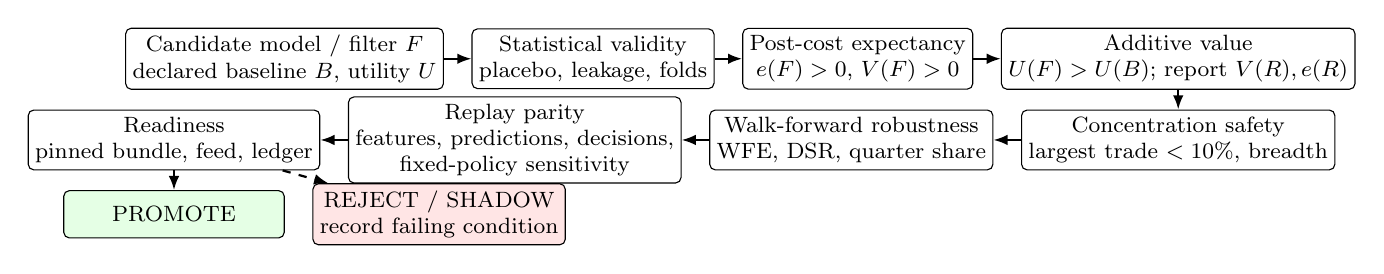
\begin{tikzpicture}[node distance=2.5mm and 3.5mm, every node/.style={font=\footnotesize}, box/.style={draw, rounded corners=2pt, minimum height=6mm, minimum width=28mm, inner sep=2.5pt, align=center}, arr/.style={-{Latex[length=1.8mm]}, thick}]
\node[box] (c) {Candidate model / filter $F$\\ declared baseline $B$, utility $U$};
\node[box, right=of c] (s) {Statistical validity\\ placebo, leakage, folds};
\node[box, right=of s] (e) {Post-cost expectancy\\ $e(F)>0$, $V(F)>0$};
\node[box, right=of e] (a) {Additive value\\ $U(F)>U(B)$; report $V(R),e(R)$};
\node[box, below=of a] (k) {Concentration safety\\ largest trade $<10\%$, breadth};
\node[box, left=of k] (r) {Walk-forward robustness\\ WFE, DSR, quarter share};
\node[box, left=of r] (p) {Replay parity\\ features, predictions, decisions,\\ fixed-policy sensitivity};
\node[box, left=of p] (d) {Readiness\\ pinned bundle, feed, ledger};
\node[box, below=of d, fill=green!10] (go) {PROMOTE};
\node[box, right=of go, fill=red!10] (no) {REJECT / SHADOW\\ record failing condition};
\draw[arr] (c) -- (s); \draw[arr] (s) -- (e); \draw[arr] (e) -- (a); \draw[arr] (a) -- (k); \draw[arr] (k) -- (r); \draw[arr] (r) -- (p); \draw[arr] (p) -- (d); \draw[arr] (d) -- (go);
\draw[arr, dashed] (d) -- (no);
\end{tikzpicture}
\caption{The \SPC\ as a sequential gate. Any failing condition stops promotion and is recorded with the CAA table that exposed it.}
\label{fig:spc}
\end{figure}

Table~\ref{tab:spc} states, for each condition, what is tested, why the condition exists, the minimum evidence, and the failure state. Thresholds are the repository's existing ones where they exist; where no defensible number exists the condition is stated as a test without a number.

\begin{table}[t]
\centering\scriptsize
\caption{The \SPC. Numeric thresholds are the repository's existing gates; conditions without a number are tests to be reported, not arbitrary limits.}
\label{tab:spc}
\begin{tabular}{@{}p{1.7cm}p{3.3cm}p{3.0cm}p{3.5cm}p{2.9cm}@{}}
\toprule
Condition & What is tested & Why it exists & Minimum evidence & Failure state \\
\midrule
\textsc{Stat} & Leakage-safe design (purge, embargo, train-only policy selection), label-shuffle placebo, enough folds and events & A filter tuned on the data it is scored on always looks good & Placebo gap $>0.03$ AP over $\ge 10$ shuffles; embargo audit with zero boundary failures; promotion-quality fold count; $\ge 3$ trades/week & Any test-window information in a cutoff, threshold, or block list; auto-relaxed folds \\
\addlinespace
\textsc{Exp} & Post-cost expectancy and net PnL of $F$ under the declared cost contract & Classifier metrics are not money & $e(F)>0$ and $V(F)>0$ on walk-forward test trades with scheduled spread, slippage, commission & $V(F)\le 0$; costs changed after the fact \\
\addlinespace
\textsc{Add} & CAA of $F$ against $B$: $U(F)$ vs $U(B)$, $V(R)$, $e(R)$, nesting, cutoff-rule sensitivity & The accepted set cannot be judged without the rejected set (Eq.~\ref{eq:identity}) & $U(F)>U(B)$ for the declared $U$; if $V(R)>0$ the record states the alpha given up and why (risk, capacity); same sign of $U(F)-U(B)$ under every decision-time cutoff rule & $\pi\uparrow$ with $U\downarrow$ (\AF); sign flips across cutoff rules; non-nested policy reported as a filter \\
\addlinespace
\textsc{Conc} & Largest-trade, top-5, top-10\% shares; side, session, regime, quarter breadth of $A$ (and of $R$) & A small $A$ can pass on a few trades; a filter can move profit into one pocket & Largest-trade share $<0.10$; profitable-quarter share $\ge 0.60$; positive-composite share $\ge 0.60$; result survives removal of the largest winner & Gate passed by $<0.001$ margin; profit in one pocket or one shock day \\
\addlinespace
\textsc{Rob} & Walk-forward stability of $F$ & A prune that fits the test tape fails forward & Sharpe $\ge 0.80$, DSR $\ge 0.30$ with recorded trials, WFE $>0.50$, drawdown $<12\%$ (advisory) & Positive net with negative WFE; DSR below limit after trial count \\
\addlinespace
\textsc{Parity} & The exact deployable policy reproduces the research decisions & The adaptive research result and the static live contract are different policies & Feature, prediction, and decision replay with zero (or documented dead-input) mismatches; fixed-policy sensitivity re-scored against the same gates; identical cutoff semantics in research and runtime code & Fixed contract fails a gate the adaptive result passed; quantile window differs between paths \\
\addlinespace
\textsc{Ready} & Artifact and operational readiness & A promotable result is not a deployable one & Immutable bundle with pinned model, scaler, calibrator, config, training summary; registered policy artifact; healthy feed; markout ledger; documented failure conditions and monitoring & Missing policy artifact; stale feed; unstarted confirmation clock \\
\bottomrule
\end{tabular}
\end{table}

\paragraph{What is already implemented.} \textsc{Exp}, \textsc{Conc}, and \textsc{Rob} are the existing eight gates; \textsc{Stat} is the promotion-quality contract plus the placebo and leakage audits; \textsc{Ready} is the paper-signal bundle and readiness audit. \textsc{Parity} exists as an audit script whose outcome is recorded next to the decision but not as a condition inside the acceptance object; the FRVP continuation case (Table~\ref{tab:parity}) shows why it must be. \textsc{Add} is the missing piece. The per-fold policy selector compares a candidate's \emph{expectancy} to the baseline's and requires only that the candidate's net PnL be positive, never that it exceed the baseline's; the quantile study compared filtered runs against the unfiltered baseline informally, and the regime-prune decisions weighed Sharpe and concentration against net PnL without a declared rule. None of these is wrong on its own; the contract makes the trade-off explicit and auditable.

\paragraph{Which metrics were misleading.} Event precision and $F_{0.5}$ were misleading for every hard-abstain pair on a profitable branch; label precision was misleading for the ES quantile filters; average precision was misleading for the breakout pilot. Per-trade expectancy was misleading whenever $V(R)>0$ but $e(R)<e(A)$ (the OTE long TCN under absolute thresholds, the FRVP continuation prune), because it hid a large positive $V(R)$. The largest-trade gate was misleading when it was passed by $0.0001$ and failed again under the fixed contract.

\section{Discussion}

\subsection{What classifier metrics still tell us}

Classifier metrics remain the right diagnostics for the model, and a discrimination floor (ROC-AUC or AP lift over the base rate) belongs in \textsc{Stat}: the branches on which quantile filters behaved erratically are precisely the ones with AUC below 0.60, and a filter cannot select what the score does not order. Where the score orders value (Figure~\ref{fig:quintiles}, left column), a threshold is a sound control and the hard-abstain rules, not the threshold, are what removed profit. The distinction the paper insists on is between a metric of the model and a criterion for promoting a decision policy.

\subsection{When abstention does help}

Abstention helped in three recognisable situations in this repository: when the baseline was net negative and the vetoes removed losing trades (FRVP long meta, OTE breakout and short-side static pairs, ICT long continuation); when a specific losing pocket was identified from breakdowns and blocked as a regime/session rule rather than a confidence rule (FRVP continuation v3, Setup-2 prune, OTE short meta prune v1); and when the utility was explicitly risk-adjusted and the rejected profit was small relative to the drawdown removed (FRVP continuation, $-42\%$ net for a 6.6-fold drawdown reduction and an accepted gate). In each case CAA would have reported $V(R)<0$, or $V(R)>0$ with a documented reason, and the contract would have promoted the policy. The failure the paper targets is not abstention but the promotion of abstention on the wrong objective.

\subsection{Limitations}

The evidence comes from one repository's saved artifacts and three related intraday strategy families; the censuses share trades and folds and are descriptive, not tests. Trade tapes exist only for the selected policy, so rejected-population economics for the hard-abstain pairs are exact in aggregate but not decomposable by rule or into concentration statistics; the per-reason attribution proposed internally was never run. The causal and rolling cutoff variants are re-screens of already-emitted trades, not full candidate-level reruns, and the rolling variant approximates the live rule (100 emitted trades versus 512 candidates). The OTE row-level label is not a precision proxy (consecutive bars inside an event zone are labelled positive), so event precision from the policy evaluations is used for OTE. The ICT continuation branches have 165--247 trades and are dominated by single trades on both sides of the comparison. Replay parity has been demonstrated on frozen bars and historical predictions, not over a live confirmation window, and one unexplained baseline drift between runs of the same model remains open.

\section{Conclusion}

A model that predicts labels better is not thereby a better trading signal, and a filter that makes the accepted trades look better is not thereby a better policy. In the saved experiments of this repository, hard regime abstains raised event precision from 0.35 to 0.99 while removing more than two-thirds of net profit, fold after fold; confidence-quantile filters removed most or all of the profit of two branches while raising their precision; and whether a quantile filter helped or hurt depended on how its cutoff was computed, which differs between the research and live code. The same evidence contains genuine successes, and the difference between the two is visible only in the rejected population. \CAA\ measures that population from artifacts a pipeline already has. The \SPC\ makes its result, together with post-cost expectancy, concentration, robustness, replay parity, and readiness, the condition for promotion. Before celebrating the trades a model rejected, measure the alpha it threw away.

\paragraph{Reproducibility.} All figures and tables are produced by \path{scripts/analyze_attribution.py} and \path{scripts/build_paper_assets.py} from saved artifacts whose paths and SHA-256 digests are listed in \path{artifacts/attribution_source_manifest.csv}; the evidence map (\path{evidence_map.csv}) links each claim to its source and confidence class.

\bibliographystyle{plainnat}
\bibliography{references}

\end{document}
